\documentclass{article}

\usepackage{graphicx}
\usepackage{tikz}
\usepackage{tikzsymbols}
\usetikzlibrary{calc,patterns,shapes.geometric}
\pagestyle{empty}
\usepackage[margin=0pt]{geometry}
\geometry{papersize={14in,12in}}

\def\centerarc[#1](#2)(#3:#4:#5){\draw[#1] ($(#2)+({#5*cos(#3)},{#5*sin(#3)})$) arc (#3:#4:#5);}

\begin{document}
	\begin{figure}
		\centering
		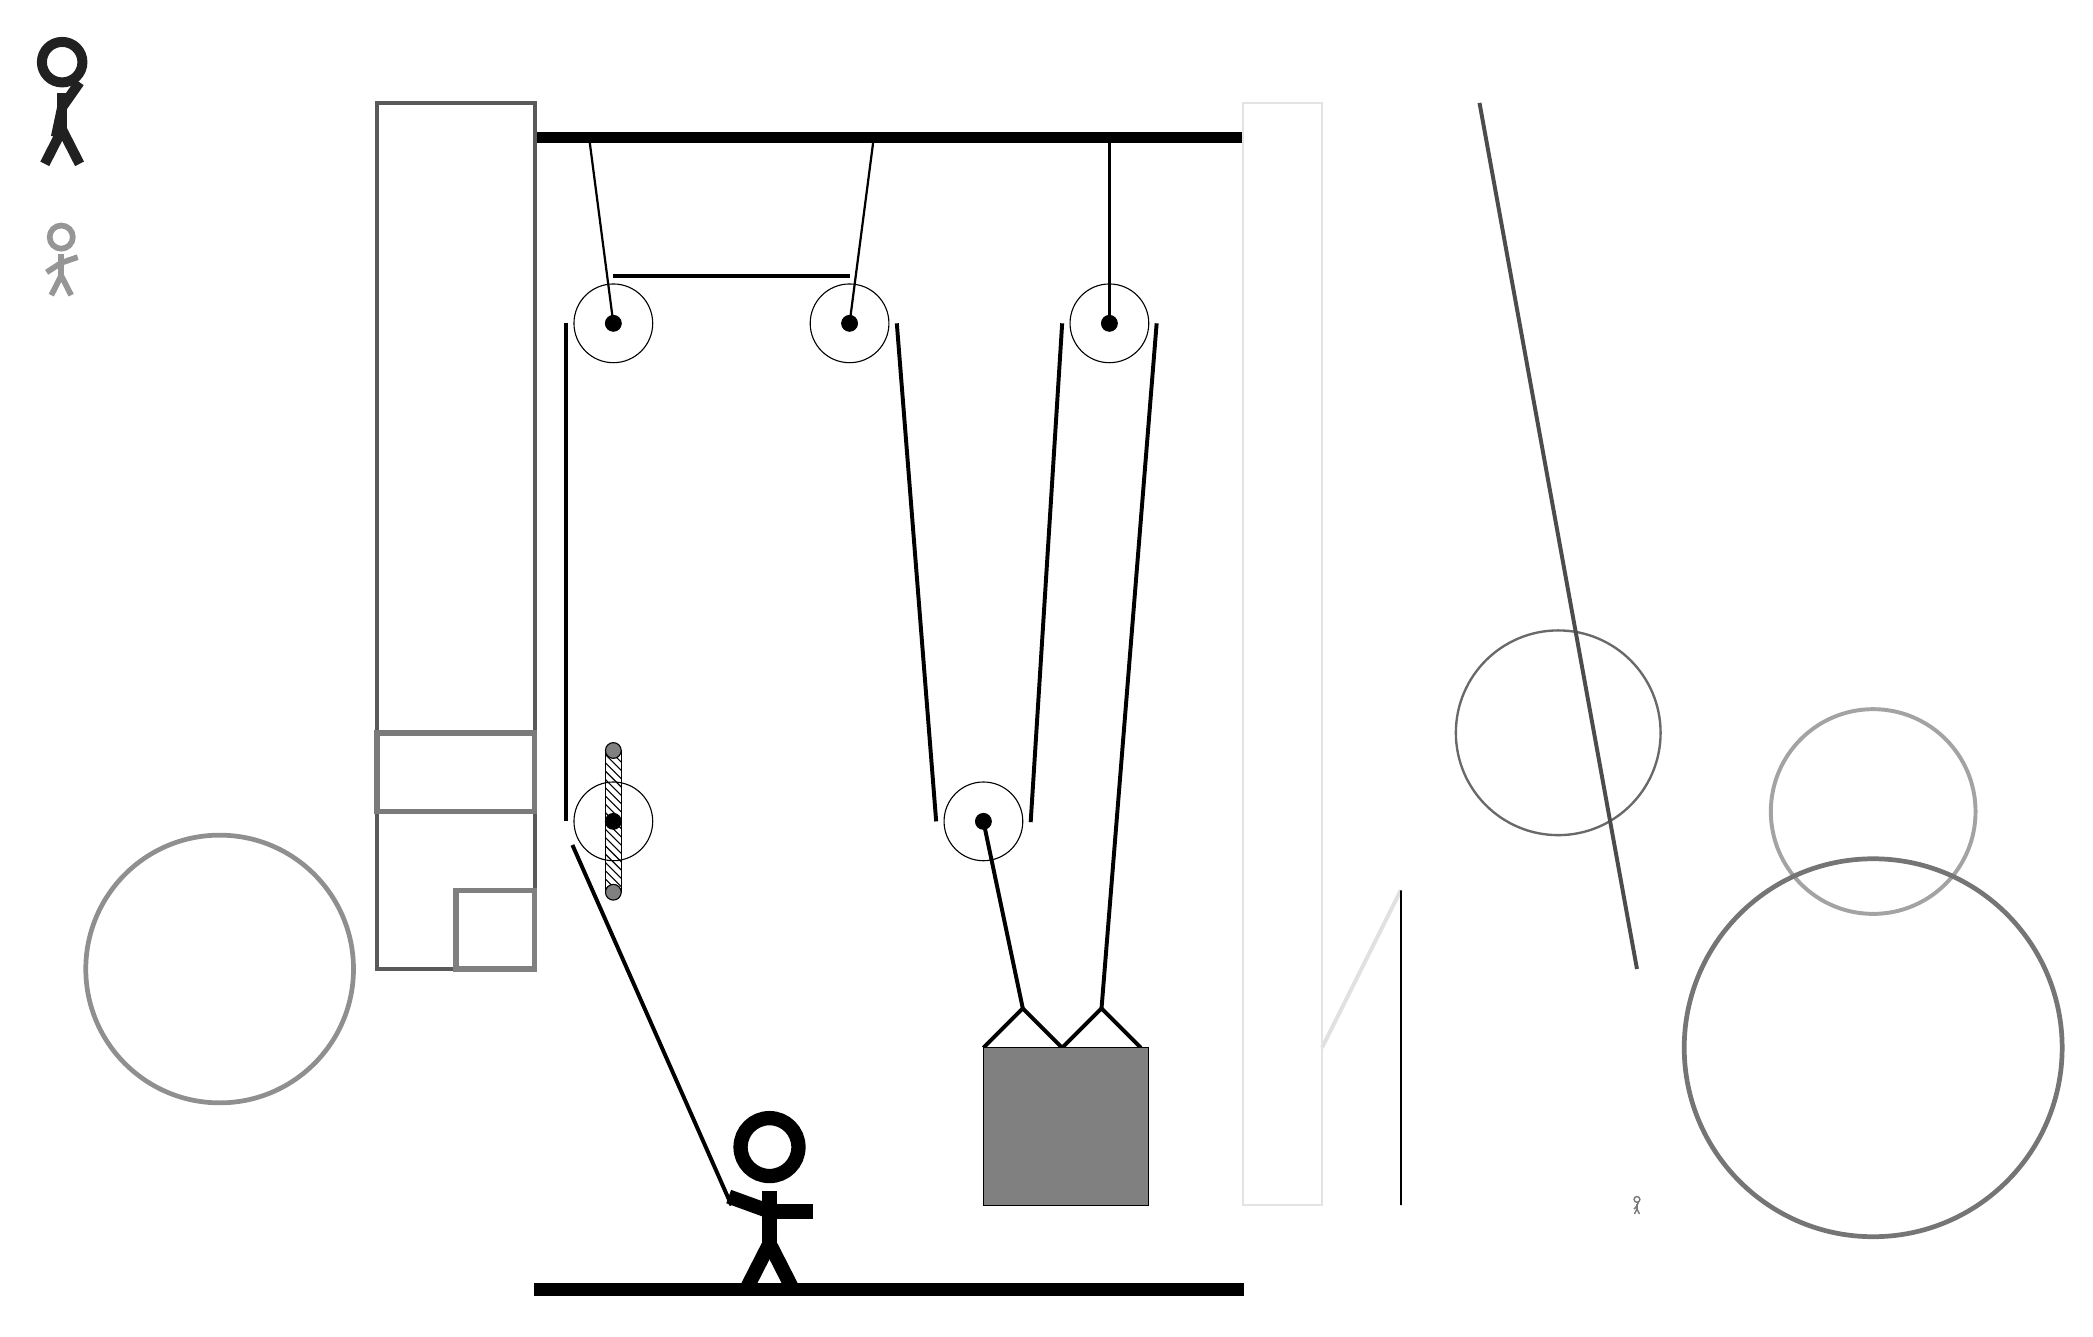
\begin{tikzpicture}
			%%%%% START %%%%%
			
			\draw[fill=black] (-3, 11.5) rectangle (6, 11.625);
			
			\draw (1, 9.2) circle (0.5);
			\draw[fill=black] (1, 9.2) circle (0.1);
			\draw[thick] (1, 9.2) -- (1.3, 11.5);
			
			\draw (4.3, 9.2) circle (0.5);
			\draw[fill=black] (4.3, 9.2) circle (0.1);
			\draw[thick] (4.3, 9.2) -- (4.3, 11.5);
			
			\draw (2.7, 2.875) circle (0.5);
			\draw[fill=black] (2.7, 2.875) circle (0.1);
			
			\draw[line width=0.5mm]  (2.7, 0.0) -- (3.2, 0.5) -- (3.7, 0.0) -- (4.2, 0.5) -- (4.7, 0.0);
			\draw[fill=black!50] (2.7, 0.0) rectangle (4.8, -2.0);
			
			\draw (-2, 9.2) circle (0.5);
			\draw[fill=black] (-2, 9.2) circle (0.1);
			\draw[thick] (-2, 9.2) -- (-2.3, 11.5);
			
			\draw (-2, 2.875) circle (0.5);
			\draw[fill=black] (-2, 2.875) circle (0.1);
			\draw[pattern=north west lines, pattern color=black] (-2.1, 3.775) rectangle (-1.9, 1.975);
			\draw[fill=black!50] (-2, 3.775) circle (0.1);
			\draw[fill=black!50] (-2, 1.975) circle (0.1);
			
			\draw[line width=0.5mm](-0.5, -2) -- (-2.5196, 2.575);
			\centerarc[line width=0.5mm](-2, 2.875)(180:210:0.6);
			\draw[line width=0.5mm](-2.6, 2.875) -- (-2.6, 9.2);
			\centerarc[line width=0.5mm](-2, 9.2)(90:180:0.6);
			
			\draw[line width=0.5mm](-2, 9.8) -- (1, 9.8);
			\centerarc[line width=0.5mm](1, 9.2)(0:90:0.6);
			\draw[line width=0.5mm](1.6, 9.2) -- (2.1, 2.875);
			\centerarc[line width=0.5mm](2.7, 2.875)(180:370:0.6);
			\draw[line width=0.5mm] (3.3, 2.865) -- (3.7, 9.2);
			\centerarc[line width=0.5mm](4.3, 9.2)(0:180:0.6);
			\draw[line width=0.5mm](4.2, 0.5) -- (4.9, 9.2);
			\draw[line width=0.5mm] (3.2, 0.5) -- (2.7, 2.875);
			
			\draw [line width=0.5mm, color=black!36](14, 3) circle (1.3);
			
			\draw [line width=0.3mm, color=black!59](10, 4) circle (1.3);
			\draw[line width=0.5mm, color=black!12](8, 2) -- (7, 0);
			\draw [line width=0.6mm, color=black!44](-7, 1) circle (1.7);
			\node[line width=0.2mm, color=black!41] at (-9, 10) {\Strichmaxerl[4][33][19]};
			
			\draw[line width=0.5mm, color=black!65] (-3, 12) rectangle (-5, 1);
			
			\node[line width=0.3mm, color=black!52] at (11, -2) {\Strichmaxerl[1][48][69]};
			\draw[line width=0.3mm, color=black!11] (7, -2) rectangle (6, 12);
			\draw[line width=0.5mm, color=black!70](9, 12) -- (11, 1);
			\draw[line width=0.2mm, color=black!100] (8, -2) rectangle (8, 2);
			\node[line width=0.3mm, color=black!87] at (-9, 12) {\Strichmaxerl[7][78][55]};
			\draw [line width=0.6mm, color=black!54](14, 0) circle (2.4);
			\draw[line width=0.7mm, color=black!52] (-3, 4) rectangle (-5, 3);
			
			\draw[line width=0.7mm, color=black!50] (-4, 1) rectangle (-3, 2);
			
			\node at (0, -2) {\Strichmaxerl[10][-20][0]};
			
			\draw[fill=black] (-3, -3) rectangle (6, -3.15);
			
			%%%%% END %%%%%
		\end{tikzpicture}
	\end{figure}	
\end{document}